%%%%%%%%%%%%%%%%%%%%%%%%%%%%%%%%%%%%%%%%%%%%%%%%%%%%%%%%%%%%%%%%%%%%%
%
% Axel Fahy
% 11.01.2017
%
%%%%%%%%%%%%%%%%%%%%%%%%%%%%%%%%%%%%%%%%%%%%%%%%%%%%%%%%%%%%%%%%%%%%%%

\documentclass[11pt]{article}
\usepackage[a4paper]{geometry}
\usepackage[utf8]{inputenc}
\usepackage[myheadings]{fullpage}
\usepackage{fancyhdr}
\usepackage{lastpage}
\usepackage{graphicx, wrapfig, subcaption, setspace, booktabs}
\usepackage[T1]{fontenc}
\usepackage[font=small, labelfont=bf]{caption}
\usepackage{fourier}
\usepackage[protrusion=true, expansion=true]{microtype}
\usepackage[english]{babel}
\usepackage{sectsty}
\usepackage{url, lipsum}
\usepackage{hyperref}
\usepackage{parskip}                                                  % Remove indentation
\usepackage{float}

%-------------------------------------------------------------------------------
% MARGIN SETTINGS
%-------------------------------------------------------------------------------
\geometry {
	paper=a4paper, % Change to letterpaper for US letter
	inner=1cm, % Inner margin
	outer=2cm, % Outer margin
	bindingoffset=1cm, % Binding offset
	top=2.5cm, % Top margin
	bottom=2.5cm, % Bottom margin
	%showframe,% show how the type block is set on the page
}

%-------------------------------------------------------------------------------
% LIST DIRECTORIES
%-------------------------------------------------------------------------------
\usepackage[dvipsnames]{xcolor}                                       % Color names
\usepackage{dirtree}                                                  % List directories
\renewcommand*\DTstylecomment{\rmfamily\color{Gray}\textsc}           % Color of comments
\renewcommand*\DTstyle{\ttfamily\textcolor{OliveGreen}}               % Color of structure
\setlength{\DTbaselineskip}{12pt}                                     % Skip between lines
\DTsetlength{1em}{1em}{0.1em}{1pt}{2pt}                               % Lines format


%-------------------------------------------------------------------------------
% CODE FORMAT - MINTED
%-------------------------------------------------------------------------------
%\usepackage{minted}
%\usepackage{etoolbox}
%\usepackage{setspace}
%\BeforeBeginEnvironment{minted}{\begin{onehalfspacing*}}
%\AfterEndEnvironment{minted}{\end{onehalfspacing*}}

%-------------------------------------------------------------------------------
% CODE FORMAT
%-------------------------------------------------------------------------------
\usepackage{listings}                                                 % Code listings
\usepackage{listingsutf8}
\lstset{inputencoding=utf8/latin1}
\usepackage{color}
\definecolor{mygreen}{rgb}{0,0.6,0}
\definecolor{mygray}{rgb}{0.5,0.5,0.5}
\definecolor{mymauve}{rgb}{0.58,0,0.82}
\definecolor{bggray}{rgb}{0.95, 0.95, 0.95}
\lstset{ %
    aboveskip=15pt,                  % space before block
    belowskip=0pt,                 % space after block, don't know why it must be negative
    backgroundcolor=\color{bggray},   % choose the background color; you must add \usepackage{color} or \usepackage{xcolor}
    basicstyle=\footnotesize,        % the size of the fonts that are used for the code
    breakatwhitespace=false,         % sets if automatic breaks should only happen at whitespace
    breaklines=true,                 % sets automatic line breaking
    captionpos=b,                    % sets the caption-position to bottom
    commentstyle=\color{mygreen},    % comment style
    deletekeywords={...},            % if you want to delete keywords from the given language
    escapeinside={\%*}{*)},          % if you want to add LaTeX within your code
    extendedchars=true,              % lets you use non-ASCII characters; for 8-bits encodings only, does not work with UTF-8
    frame=single,                    % adds a frame around the code
    frameround=tttt                  % tttt for having the corner round.
    keepspaces=true,                 % keeps spaces in text, useful for keeping indentation of code (possibly needs columns=flexible)
    keywordstyle=\color{blue},       % keyword style
    language=,                 % the language of the code
    morekeywords={*,...},            % if you want to add more keywords to the set
    numbers=left,                    % where to put the line-numbers; possible values are (none, left, right)
    numbersep=5pt,                   % how far the line-numbers are from the code
    numberstyle=\tiny\color{mygray}, % the style that is used for the line-numbers
    rulecolor=\color{black},         % if not set, the frame-color may be changed on line-breaks within not-black text (e.g. comments (green here))
    showspaces=false,                % show spaces everywhere adding particular underscores; it overrides 'showstringspaces'
    showstringspaces=false,          % underline spaces within strings only
    showtabs=false,                  % show tabs within strings adding particular underscores
    stepnumber=1,                    % the step between two line-numbers. If it's 1, each line will be numbered
    stringstyle=\color{mymauve},     % string literal style
    tabsize=2,                       % sets default tabsize to 2 spaces
    title=\lstname                   % show the filename of files included with \lstinputlisting; also try caption instead of title
}
%-------------------------------------------------------------------------------
% COMMAND LINE FORMAT
%-------------------------------------------------------------------------------
\lstdefinestyle{CommandLineStyle}{
    backgroundcolor=\color{black},
    basicstyle=\color{white}\footnotesize\ttfamily,
    breakatwhitespace=false,
    breaklines=true,
    captionpos=b,
    deletekeywords={...},
    escapeinside={\%*}{*)},
    extendedchars=true,
    frame=none,
    keepspaces=true,
    numbers=none,
    rulecolor=\color{black},
    showspaces=false,
    showstringspaces=false,
    showtabs=false,
    tabsize=2,
    deletekeywords={default}
}
%-------------------------------------------------------------------------------
% INLINE FORMAT
%-------------------------------------------------------------------------------
\lstdefinestyle{InlineStyle}{
    basicstyle=\footnotesize,
    breakatwhitespace=false,
    breaklines=true,
    captionpos=b,
    deletekeywords={...},
    escapeinside={\%*}{*)},
    extendedchars=true,
    frame=none,
    keepspaces=true,
    keywordstyle=\color{blue},
    language=java,
    morekeywords={*,...},
    showspaces=false,
    showstringspaces=false,
    showtabs=false,
    tabsize=2,
}

%-------------------------------------------------------------------------------
% CODE FORMAT
%-------------------------------------------------------------------------------
\definecolor{codegray}{gray}{0.9}
\newcommand{\code}[1]{{\texttt{#1}}}
\newcommand{\codeg}[1]{\colorbox{codegray}{\texttt{#1}}}
\newcommand{\HRule}[1]{\rule{\linewidth}{#1}}
\newcommand{\address}[1]{{\texttt{#1}}}

\onehalfspacing
\setcounter{tocdepth}{5}
\setcounter{secnumdepth}{5}


% Remove the 'Chapter' before each chapter.
%\usepackage{titlesec}
%\titleformat{\chapter}{}{}{0em}{\bf\LARGE}

%\makeatletter
%\renewcommand{\@makechapterhead}[1]{%
%\vspace*{0 pt}%
%\bfseries\Huge\thechapter.\ #1
%\par\nobreak\vspace{40 pt}}}
%\makeatother

%-------------------------------------------------------------------------------
% HEADER & FOOTER
%-------------------------------------------------------------------------------
\pagestyle{fancy}
\fancyhf{}
\setlength\headheight{15pt}
\fancyhead[L]{Axel Fahy \& Rudolf Höhn}
%\fancyhead[R]{\textsl{SRE}}
\fancyfoot[R]{\textsl{Page \thepage\ of \pageref{LastPage}}}

%-------------------------------------------------------------------------------
% TITLE PAGE
%-------------------------------------------------------------------------------
\title{\vspace{-2cm}LoRaFall\\Internet of Things}
\author{Axel Fahy \& Rudolf Höhn}
\date{\today}

\begin{document}
\maketitle

\thispagestyle{empty} % Remove the number on page title.
%\newpage
%\tableofcontents
%\newpage


%-------------------------------------------------------------------------------
% Section title formatting
\sectionfont{\scshape}
%-------------------------------------------------------------------------------

%-------------------------------------------------------------------------------
% BODY
%-------------------------------------------------------------------------------
\section{Introduction}

The aim of the project is to develop an application using the \textit{Bluetooth Low Energy} and \textit{LoRa} technologies. The project consists at developing a system that can detect when someone is falling. It can also alert other devices of a fall.

%-------------------------------------------------------------------------------
%-------------------------------------------------------------------------------
\section{Architecture}

Here is the architecture of the project.

\begin{figure}[H]
    \centering
    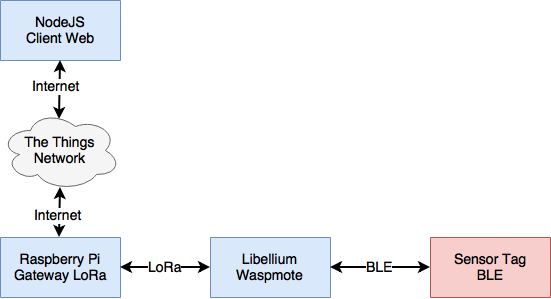
\includegraphics[scale=0.6]{architecture_iot_lora_project.png}
    \caption{Architecture of the project}
\end{figure}

\section{Features}

We are able to detect different status on the BLE device, such as wait, walk, run and fall. Then, the status is sent to the LoRaWAN using a gateway. The waspmotes are registered into The Things Networks and we are able to see the uplink and downlink message on their GUI. Speaking of downlink messages, if the waspmote receive a downlink message when it sent a message, the buzzer ring and the led turns on to indicate that someone has fallen. This downlink is sent from the NodeJS client using the ttn API. The devices are dynamically added or deleted from the GUI. They are displayed on the webpage with their status and a button allowing sending them a downlink message. The GUI is presented in the figure~\ref{fig:web}.

\begin{figure}[h]
    \centering
    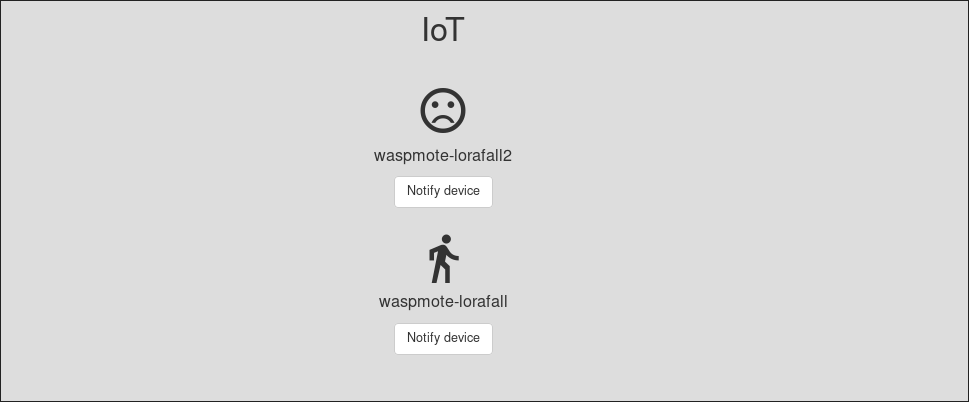
\includegraphics[scale=0.6]{website_image.png}
    \caption{Webpage with two devices}
    \label{fig:web}
\end{figure}


%-------------------------------------------------------------------------------
%-------------------------------------------------------------------------------
\section{Technologies used}

\begin{itemize}
    \item Waspmote
    \item Bluetooth Low Energy
    \item LoRa technologies
    \item NodeJS
    \item The Things Network API
\end{itemize}

\section{Issues encountered}

We encountered some issues with \textit{The Things Network}. For some time, we were not able to receive any message on \textit{The Things Network} and had to reconfigure the gateway, remove the device and add it again. Moreover, we often needed to reset the \textit{frame counter} of the devices on the \textit{The Things Network} website in order to be able to receive messages. For these reasons, we would not consider using this platform for a project in production, since it is not stable enough.

\section{Acknowledgements}

We would like to express our deepest gratitude to the assistant of the course, David, for his help during this project even when it was late or during the weekend.

\end{document}
